\section{写在开始前}

在开始前,我想先解释一下本文中两个名词『DDPM』与『基于扩散的图像生成模型』之间的差异,以解释本文内容与标题之间的联系。
本文中的『DDPM』指的是文章Denoising Diffusion Probabilistic Model\cite{hoDenoisingDiffusionProbabilistic2020a}中提出的模型,是最早的『基于扩散的图像生成模型』。
而『基于扩散的图像生成模型』指的是以所有扩散过程与逆扩散过程作为基本原理的图像生成模型。
本文的标题为『基于扩散的图像生成模型与DDPM原理』,实际上是在介绍两个部分,其一为『基于扩散的图像生成模型』,其二为『DDPM原理』。第一部分将接受当前所有的『基于扩散的图像生成模型』的总体工作流程,从整体的角度为各位介绍该类模型的生成过程。第二部分以最简单的『基于扩散的图像生成模型』,也即DDPM作为基础,为各位推导最简单的流程。

下面开始第一部分,介绍『基于扩散的图像生成模型』的基本流程。

\section{基于扩散的图像生成模型的基本流程}

该部分介绍基于扩散的图像生成模型的基本工作流程,为不了解该类模型的读者简单介绍一下模型的生成过程,为后面详细介绍原理做准备。

首先需要明确的是『扩散过程与逆扩散过程』与『基于扩散的图像生成模型』这两个名词之间的差别。有些文章可能将这两个概念混淆,或直接称『基于扩散的图像生成模型』为『扩散模型』,但本文希望能将这两个概念进行辨析,以获得更明确无歧义的阅读体验。

『扩散过程与逆扩散过程』可以分成两个过程,即『扩散过程』与『逆扩散过程』。『扩散过程』其实是一个物理过程,图像生成模型中模仿这个概念,让噪声逐渐扩散到整个图像的过程被称为『扩散过程』;而『逆扩散过程』则是将扩散过程反过来,从噪声图像中恢复出一张不带有噪声的图像的过程。扩散过程可以看作『基于扩散的图像生成模型』中的一个基本原理。

而『基于扩散的图像生成模型』则是以『扩散过程与逆扩散过程』作为基本原理,进行图像生成的模型,二者是包含与被包含的关系。后者包含前者,而前者作为后者的一部分,为后者提供服务。本文中对于『扩散过程与逆扩散过程』与『基于扩散的图像生成模型』这两个概念均与上述描述保持一致,若在阅读中出现概念对这两个概念混淆的现象,可以翻阅本段文字或查阅\ref{sec_noun}名词解释部分作为参考。

其次需要介绍的是『基于扩散的图像生成模型』的输入与输出。该类模型接收对于图像的文字描述作为输入,并输出一张或多张与输入文字描述相符合的图像,如下图\ref{fig_ioput_of_model}所示。

\begin{figure}[htbp]
    \centering
    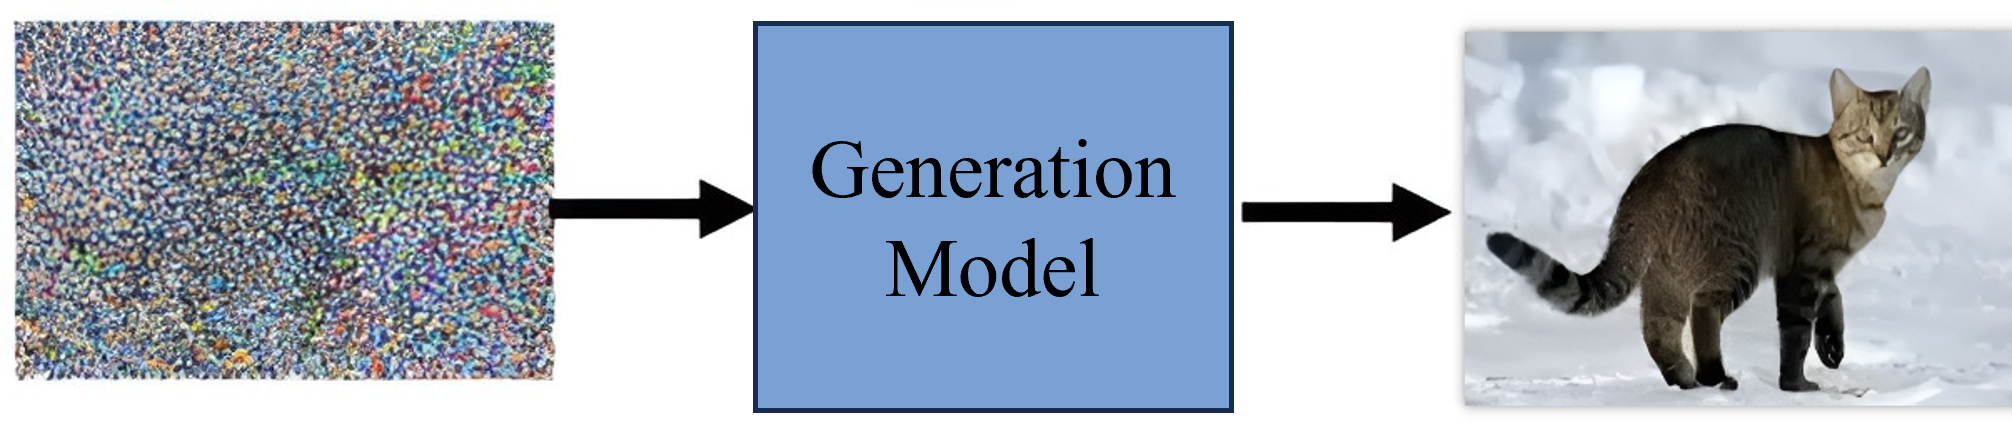
\includegraphics[width=0.8\textwidth]{figs/color/ioput_of_model.png}
    \caption{基于扩散的图像生成模型:输入与输出}
    \label{fig_ioput_of_model}
\end{figure}

当接收到文字输入后,『基于扩散的图像生成模型』将随机从高斯分布中采样一张噪声图像,并将该噪声图像与文字输入一同送进Denoise模块中。Denoise模块将去除噪声图像中的部分噪声,从而得到一张部分降噪的图像。这个过程如下图\ref{fig_denoise}所示。

\begin{figure}[htbp]
    \centering
    \subfigure[Denoise模块的输入与输出]{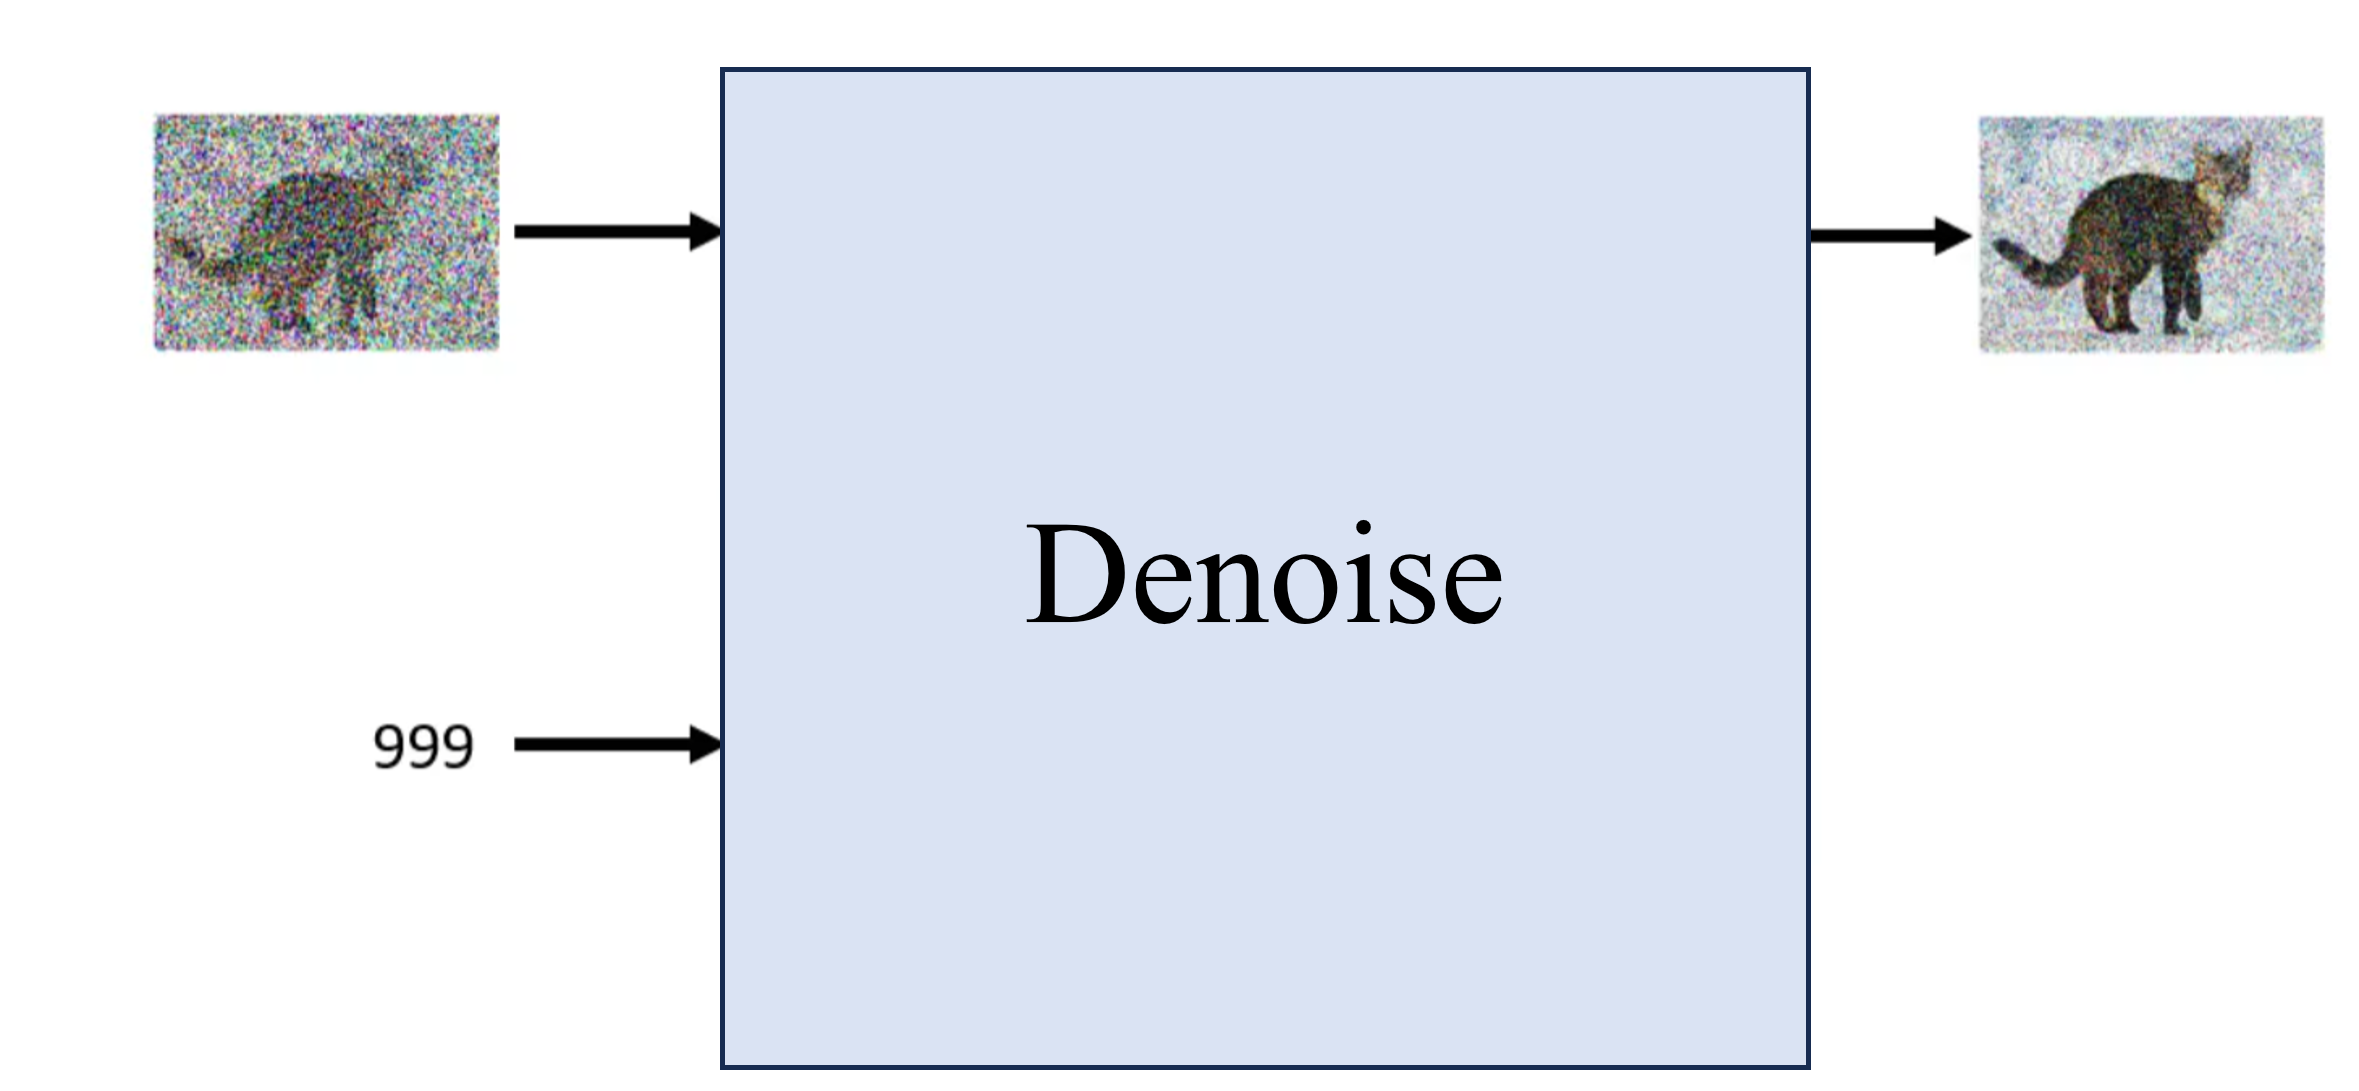
\includegraphics[width=0.4\textwidth]{figs/color/denoise.png}}
    \subfigure[单个Denoise过程]{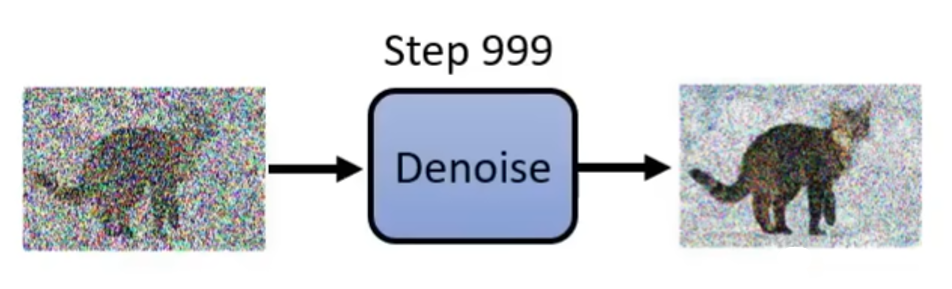
\includegraphics[width=0.4\textwidth]{figs/color/denoise1.png}}
    \caption{基于扩散的图像生成模型:Denoise模块}
    \label{fig_denoise}
\end{figure}


将得到的部分降噪图像重新输入到Denoise模块中,重复多次,便可得到一张符合输入文字描述的图像。这就是『基于扩散的图像生成模型』的基本工作流程,如图\ref{fig_process_of_model}所示。

\begin{figure}[htbp]
    \centering
    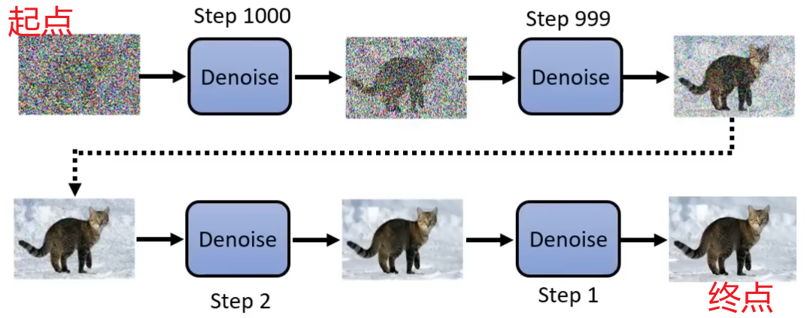
\includegraphics[width=0.8\textwidth]{figs/color/process.png}
    \caption{基于扩散的图像生成模型:整体工作流程。用一句话概括上述对『基于扩散的图像生成模型』工作流程的描述:『基于扩散的图像生成模型』接收对于图像的描述作为输入,对自己生成的一张噪声图经过多次去噪操作后,得到一张与输入文字描述相同的图像。}
    \label{fig_process_of_model}
\end{figure}

总结一下,『基于扩散的图像生成模型』接收对于图像的描述作为输入,对自己生成的一张噪声图经过多次去噪操作后,得到一张与输入文字描述相同的图像。


